%\section{Appendix}
\section{Sampling accumulation curves}

\begin{center}
	\begin{figure}[H]
		\subfloat[Species per locality]{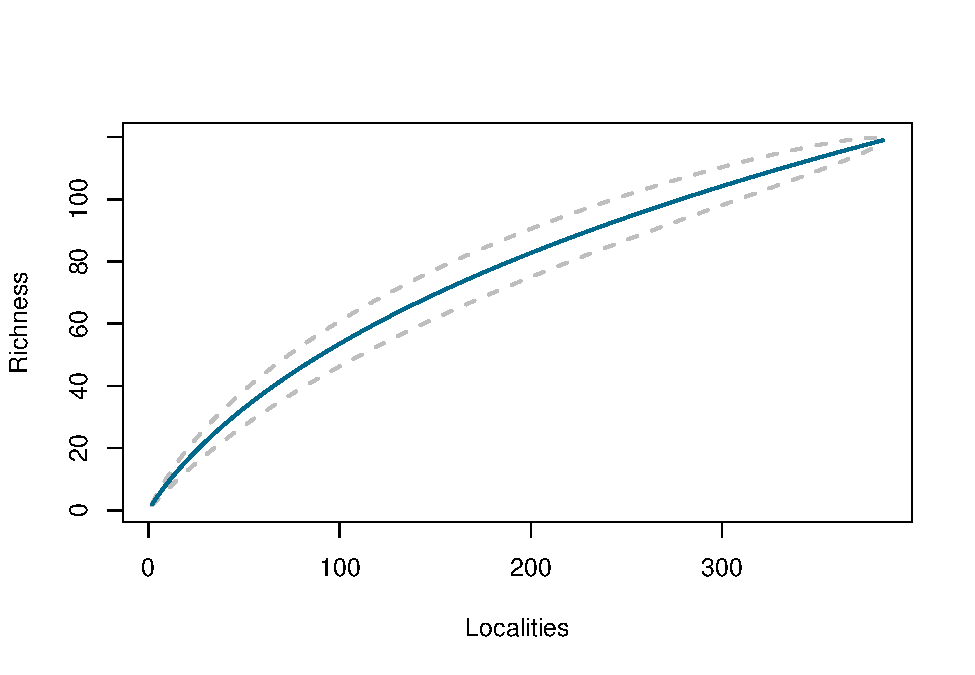
\includegraphics[scale=0.3]{MA_JJ_files/figure-latex/SACSpecies-1.pdf}}
		\subfloat[Species per reference]{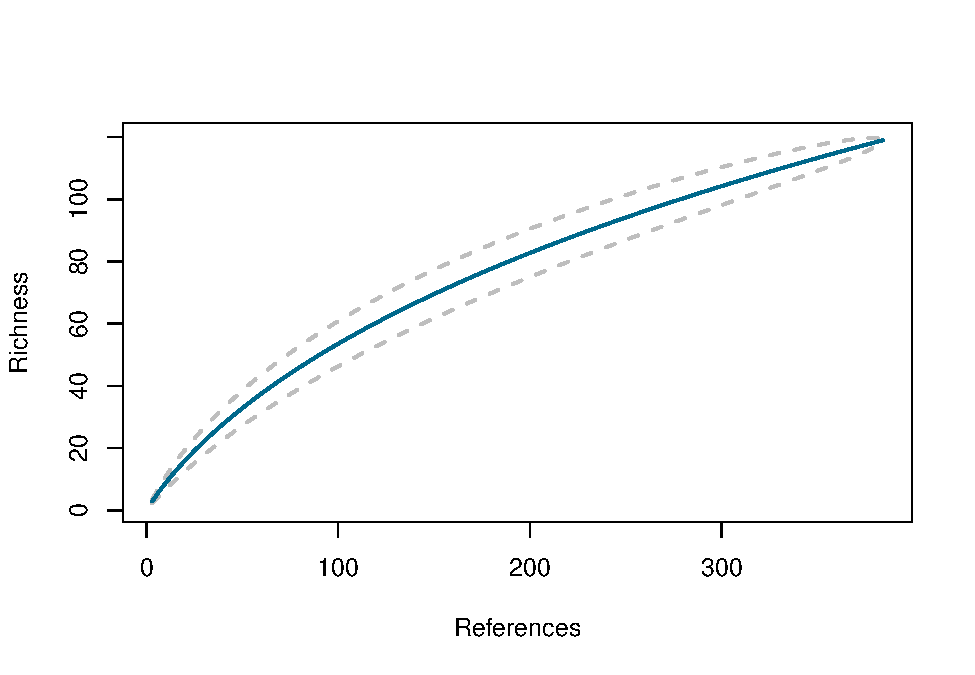
\includegraphics[scale=0.3]{MA_JJ_files/figure-latex/SACSpecies-2.pdf}}	\subfloat[Africa]{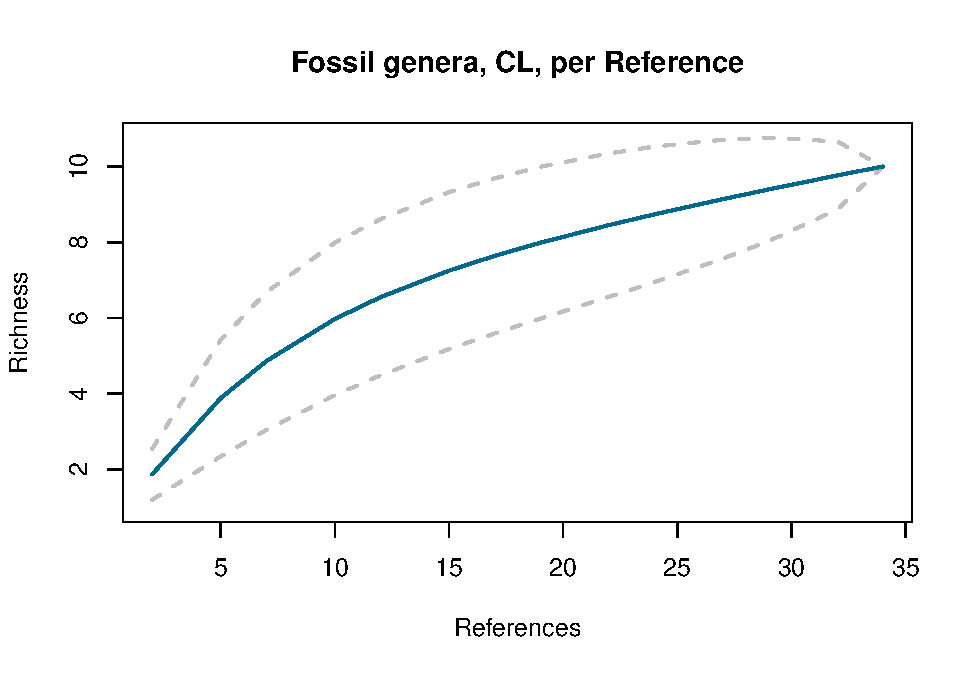
\includegraphics[scale=0.3]{MA_JJ_files/figure-latex/SACGAfrica-1.pdf}}
		\hfill %
		\subfloat[America]{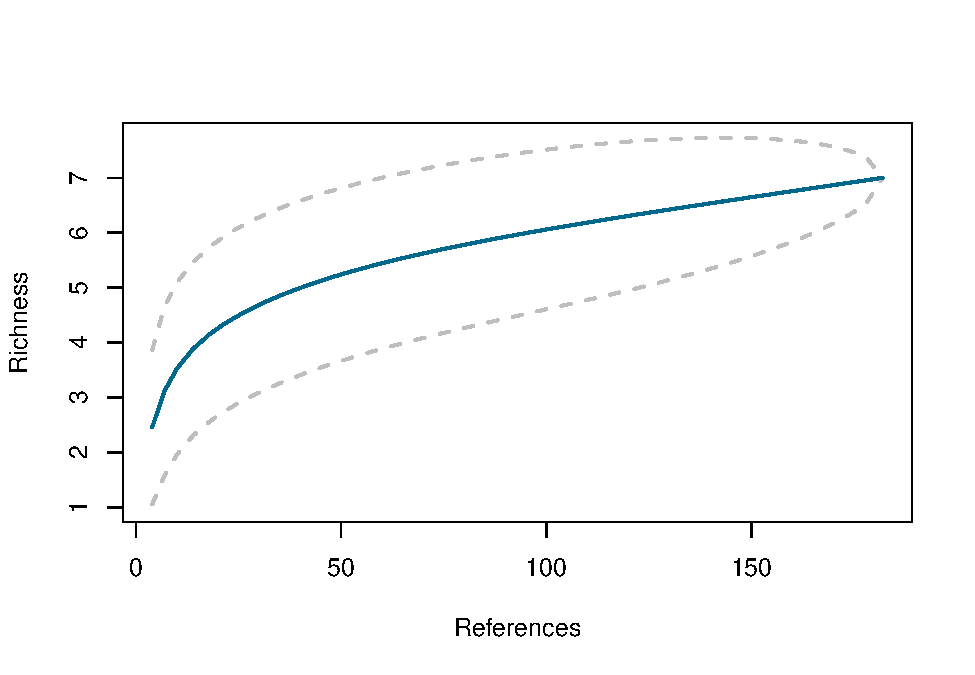
\includegraphics[scale=0.3]{MA_JJ_files/figure-latex/SACGAmerica-1.pdf}}
		\subfloat[North America]{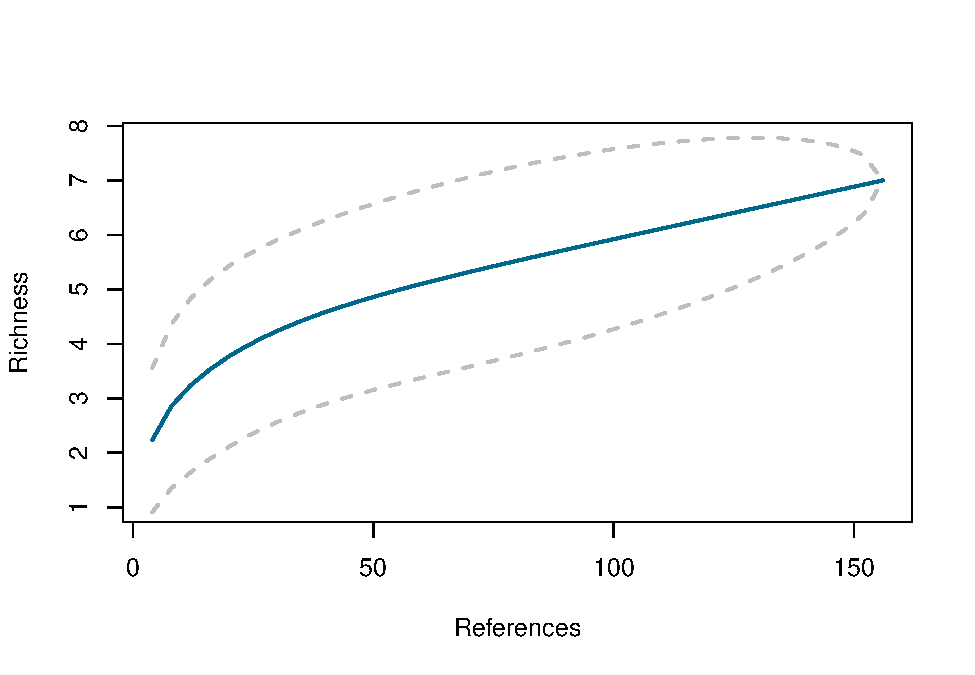
\includegraphics[scale=0.3]{MA_JJ_files/figure-latex/SACGNAmerica-1.pdf}}
		\subfloat[South America]{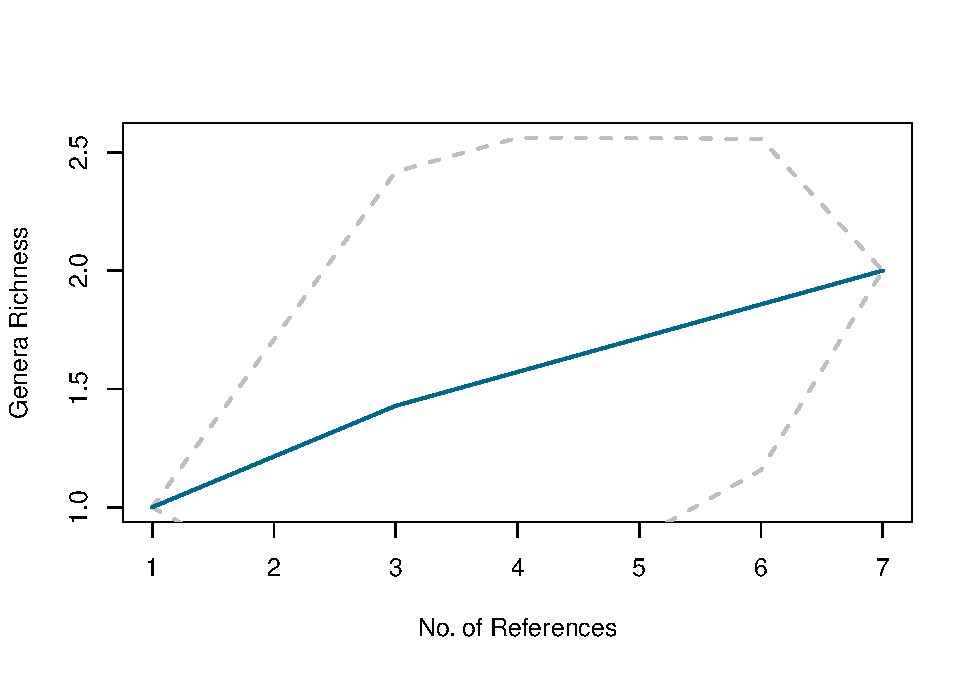
\includegraphics[scale=0.3]{MA_JJ_files/figure-latex/SACGSAmerica-1.pdf}}
		\hfill %
		\subfloat[Asia]{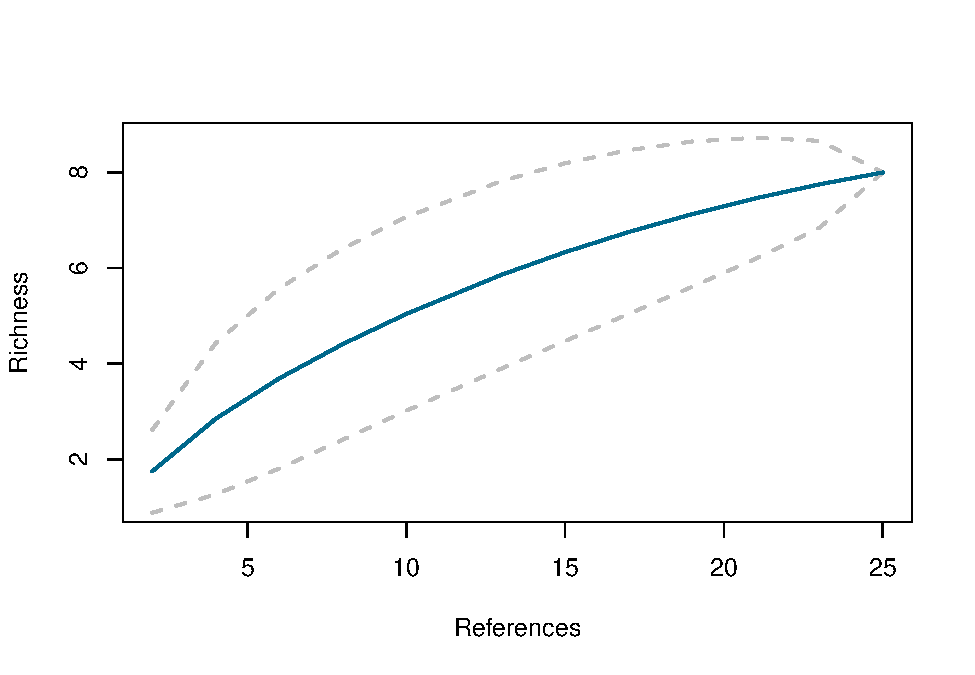
\includegraphics[scale=0.3]{MA_JJ_files/figure-latex/SACGAsia-1.pdf}}
		\subfloat[Europe]{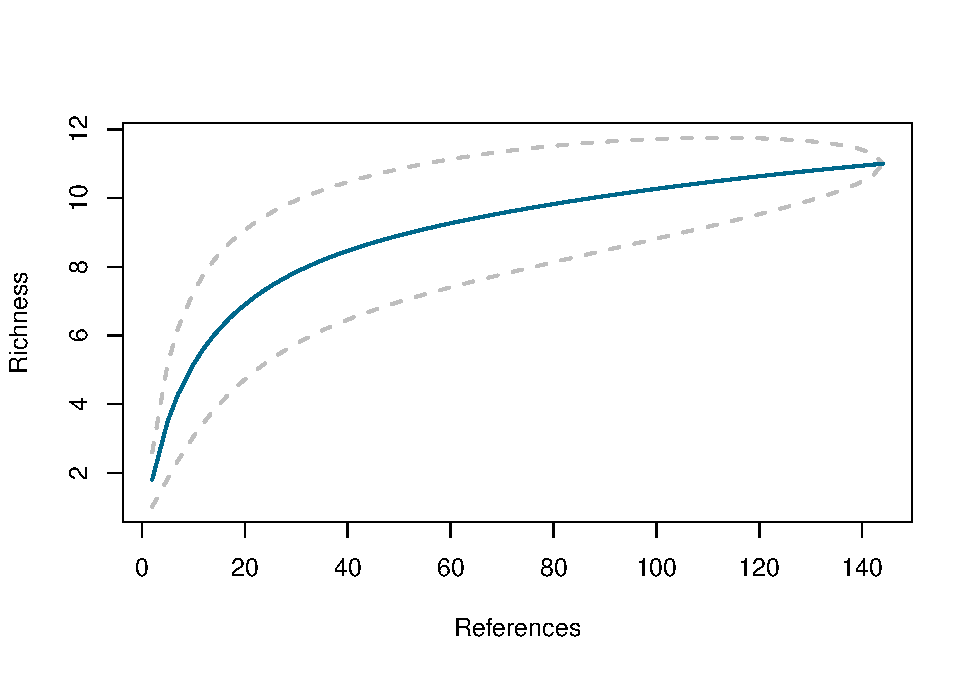
\includegraphics[scale=0.3]{MA_JJ_files/figure-latex/SACGEurope-1.pdf}}
		\subfloat[Eurasia]{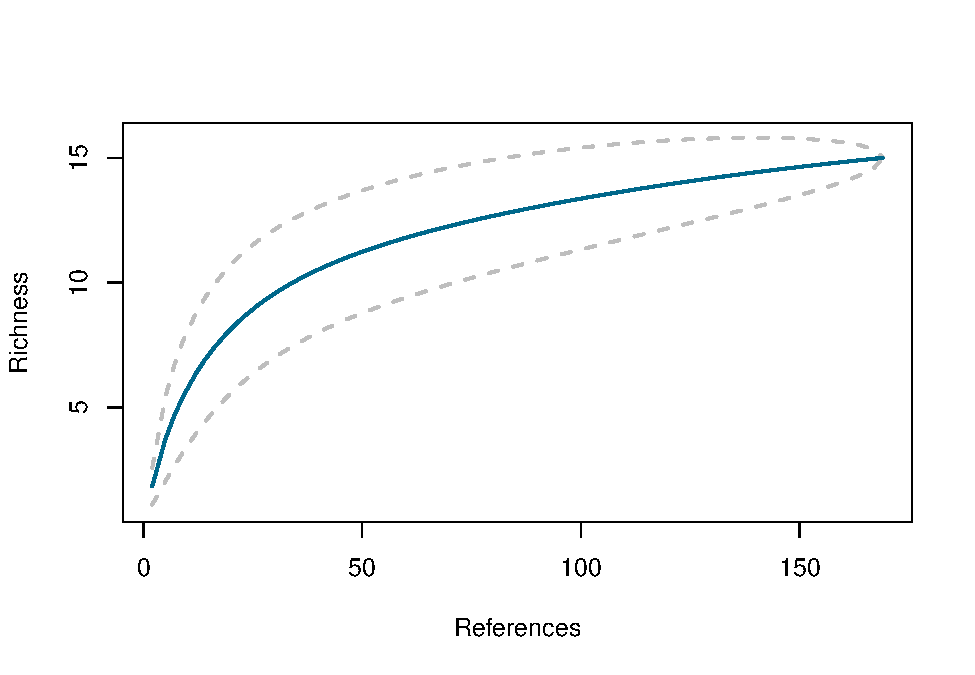
\includegraphics[scale=0.3]{MA_JJ_files/figure-latex/SACGEurasia-1.pdf}}
		\caption[Additional sampling accumulation curves]{Sampling accumulation curves: (a) - (b) Species are not sufficiently sampled, regardless of sampling unit. (c) - (i) Sampling Accumulation Curves on generic level per continent. Only Europe (h) and Eurasia (i) are sufficiently sampled. Dashed lines represent the confidence interval.}
		\label{fig:SACall}
	\end{figure}
\end{center}

\FloatBarrier


\begin{longtable}[]{@{}llllllll@{}}
	\caption{Genera abundance across the continents.}
	\label{tab:SAC}
	\toprule
	Genus & Africa.x & America & N-America & S-America & Asia.x & Europe.x &
	n\tabularnewline
	\midrule
	\endhead
	Aldabrachelys & 4 & - & - & - & 2 & - & 2\tabularnewline
	Caudochelys & - & 4 & 4 & - & - & - & -\tabularnewline
	Centrochelys & 2 & - & - & - & - & 12 & 12\tabularnewline
	Cheirogaster & - & - & - & - & - & 9 & 9\tabularnewline
	Chelonoidis & - & 28 & - & 6 & - & - & -\tabularnewline
	Ergilemys & - & - & - & - & 2 & 3 & 4\tabularnewline
	Eurotestudo & - & - & - & - & - & 10 & 10\tabularnewline
	Geochelone & 4 & 10 & 8 & 1 & 1 & 2 & 3\tabularnewline
	Gopherus & - & 92 & 88 & - & - & - & -\tabularnewline
	``Hadrianus'' & - & - & - & - & - & 1 & 1\tabularnewline
	Hesperotestudo & - & 46 & 43 & - & - & - & -\tabularnewline
	Homopus & 1 & - & - & - & - & - & -\tabularnewline
	Impregnochelys & 1 & - & - & - & - & - & -\tabularnewline
	Indotestudo & - & - & - & - & 1 & - & 1\tabularnewline
	Kinixys & 1 & - & - & - & - & - & -\tabularnewline
	Manouria & - & - & - & - & 2 & - & 2\tabularnewline
	Megalochelys & - & - & - & - & 12 & - & 12\tabularnewline
	Mesocherus & 5 & - & - & - & - & - & -\tabularnewline
	Namibchersus & 9 & - & - & - & - & - & -\tabularnewline
	Paleotestudo & - & - & - & - & - & 26 & 26\tabularnewline
	Psammobates & 1 & - & - & - & - & - & -\tabularnewline
	Stylemys & - & 1 & 1 & - & - & - & -\tabularnewline
	Taraschelon & - & - & - & - & - & 1 & 1\tabularnewline
	Testudo & 5 & 1 & 1 & - & 4 & 51 & 54\tabularnewline
	Titanochelon & - & - & - & - & - & 22 & 22\tabularnewline
	gen. & - & - & - & - & 1 & 7 & 8\tabularnewline
	\bottomrule
\end{longtable}
